\documentclass[11pt,a4paper]{article}

\usepackage{url,,}
\usepackage{graphicx}
\usepackage{hyperref}
\usepackage{amsfonts}
\usepackage{amssymb}
\usepackage{amsmath}
\usepackage{amsfonts}
\usepackage{amssymb}
\usepackage{amsmath}
\usepackage{multirow}
\usepackage{listings}
\usepackage{fullpage}
\usepackage{fancyhdr,a4wide}
\usepackage{makeidx}
\usepackage{placeins}
\usepackage[procnames,noindent]{lgrind}

\lstset{ %
language=VHDL,                % choose the language of the code
basicstyle=\footnotesize,       % the size of the fonts that are used for the code
showstringspaces=false,         % underline spaces within strings
%numbers=left,                   % where to put the line-numbers
%numberstyle=\footnotesize,      % the size of the fonts that are used for the line-numbers
%stepnumber=1,                   % the step between two line-numbers. If it's 1 each line will be numbered
%numbersep=5pt,                  % how far the line-numbers are from the code
%backgroundcolor=\color{white},  % choose the background color. You must add \usepackage{color}
showspaces=false,               % show spaces within strings adding particular underscores
showtabs=false,                 % show tabs within strings adding particular underscores
escapeinside={\%*}{*)}          % if you want to add a comment within your code
}

\begin{document}	

\begin{titlepage}

\thispagestyle{fancy}
\lhead{}
\chead{
\large{\textit{
Informatics and Mathematical Modelling\\
Technical University of Denmark}}}
\rhead{}
\rule{0pt}{50pt}
\vspace{3cm}

\begin{center}

 	\huge{\textbf{02207 : Advanced Digital Design Techniques}}\\
 	\vspace{1cm}
 	\huge{Design for Low Power by Reducing Switching Activity}\\
 	\vspace{1cm}
 	\huge{\textit{LAB 2}}\\
 	\vspace{1cm}
 	\huge{Group \textit{dt07}}\\
\end{center}

\vspace{4cm}

\begin{flushright}
	\LARGE{Markku Eerola (s053739)}\\
	\vspace{0.3cm}
	\LARGE{Rajesh Bachani (s061332)}\\
	\vspace{0.3cm}
	\LARGE{Josep Renard (s071158)}\\
\end{flushright}
\cfoot{\today}
\end{titlepage}

%\begin{abstract}
%\centering
%Abstract to be created.
%\end{abstract}

%-----------------------------------------------------------
\newpage 
\tableofcontents

\newpage 
\section{Introduction}

The purpose of this exercise was to estimate the power dissipation in a digital circuit due to the switching activity in the cells. Power is dissipated in a digital circuit, dynamically, in two ways; one, the power that is spent in charging or discharging the capacitance load connected to the output of the cell, and two, the power dissipated inside the cell due to short circuit currents and the internal capacitance charging or discharging. This holds for combinational cells. For sequential cells, there is extra power spent at every clock cycle, even if the output of the cell does not change. This is because there is some reaction to every clock cycle in sequential cells, which would take some power. 

Static power in digital circuits is due to the internal leakage currents in CMOS. Though, in this exercise, we are particularly interested in analyzing the dynamic power dissipation.

We estimate the dynamic power in a serial to parallel converter. The converter takes in 8 bits (one byte) in every clock cycle, and gives out 32 bits (4 bytes) after every 4 clock cycles. The input byte at the first clock cycle is the most significant byte in the output, whereas the input byte in the fourth clock cycle is the lowest significant byte. The converter, thus, waits for four clock cycles to produce an output. We refer to the register holding the most significant byte in the output as the most significant register, and that holding the least significant byte as the least significant register.

The report is organized as follows. In section \ref{section:designs}, we discuss three designs for a serial to parallel converter. In section \ref{section:simulation}, we simulate the VHDL code for the designs using Modelsim, and verify that all the designs are working correctly. Section \ref{section:power} contains the power results obtained from the synthesis of the VHDL using Design Vision, and Synopsys VSS for annotating the switching activity in a given time period. In this section, we discuss and justify the results obtained. Later, in section \ref{section:impl}, the VHDL is provided, alongwith the power reports from Design Vision. 

\subsection{Authors by Section}
\begin{itemize}
\item \textit{Markku Eerola} 
\item \textit{Josep Renard} 
\item \textit{Rajesh Bachani} 
\end{itemize}

\newpage
\section{Designs for Serial to Parallel Conversion}
\label{section:designs}
In this section, we give an overview of the three designs for serial to parallel conversion, which are evaluated for their power consumption in this exercise.

\subsection{Design A: Shift Register}

\begin{figure}[htp]
\centering
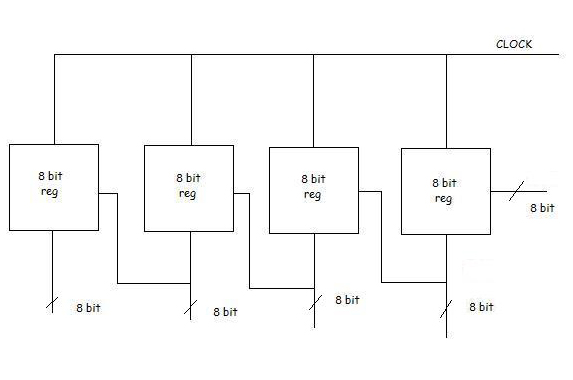
\includegraphics[width = 3.5in]{./images/shiftregister.jpg}
\caption{Converter using a 8-bit Shift Register}
\end{figure}

As we can see in Figure 1, the input data flows continuously through the registers. On every rising clock edge each of the 8-bit registers takes on a new state. The rightmost register takes its state from the input of the whole shiftregister block and all the other registers take their states from the outputs of the previous register. This can be seen as the 8-bit registers shifting the input eight bits from right to left as the next eight bits of the 32-bit word are taken in, until after four clock cycles the outputs of the registers form the whole 32-bit word which is readable from the block's output. All components of this block are driven with the same clock signal, which ensures that the 8-bit registers change their state at the same time and no data is lost. 


\subsection{Design B: Register with Enable}

\begin{figure}[htp]
\centering
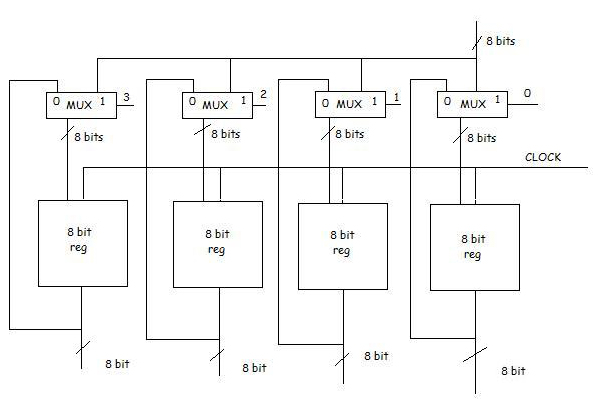
\includegraphics[width = 3.5in]{./images/shiftregisterenable.jpg}
\caption{Converter using 8-bit Registers with Enable}
\end{figure}

In Figure 2 we see another design for a serial to parallel converter. In this design we use multiplexors to control when the 8-bit registers should take on a new state. The multiplexors are controlled by enable signals generated from a 2-bit counter. The multiplexors take in two inputs, one from the output of the 8-bit register the multiplexor contols and one from the input of the whole shiftregister block. When a multiplexor is enabled by an enable signal it lets through the data from the block input, otherwise it lets through the data from the 8-bit register output. This way we can make the 8-bit registers change their state only when the bits which that particular register is supposed to put to the output of the whole block come in from the input. The 8-bit registers still operate on each rising clock edge, but since their state remains the same they consume less power in this activity. Of course the multiplexors and the logic for the enable signals consume power as well, and in this case we expect the consumption from the multiplexors and the logic to exceed the power savings from restricting the number of state changes.

\subsection{Design C: Register with Clock-Gating}

\begin{figure}[htp]
\centering
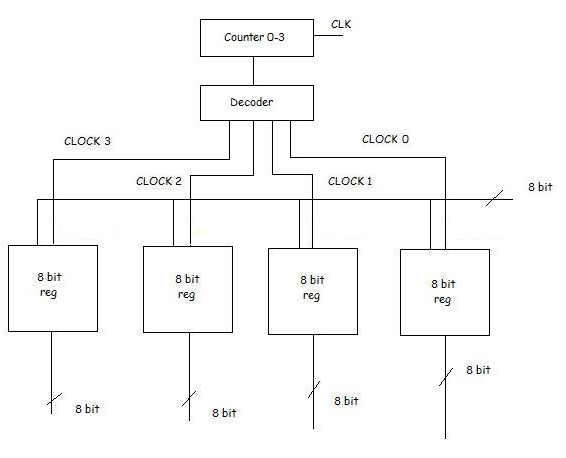
\includegraphics[width = 3.5in]{./images/shiftregistergated.jpg}
\caption{Converter using 8-bit Registers with Clock Gating}
\end{figure}

In Figure 3 we see the third and last design for a serial to parallel converter we used in the exercise. In this design we restirct the the amount of register state changes by not driving the 8-bit registers with the clock directly but instead using a 2-bit counter and a decoder to give a rising clock edge only to one 8-bit register at a time. We time these rising edges so, that when the bits which a particular 8-bit register is supposed to put to the output of the whole block come in from the input, then a rising edge is given to that 8-bit register and it will change its state. In this design the 8-bit registers operate only when they change their state on every fourth clock cycle. This means that they consume much less power. Of course the logic for dividing the clock consumes power as well, but we expect that the power savings which are gained by reducing the operation of the 8-bit registers outweighs this, since we're not only restricting the number of state changes but we're completely removing the ``idle'' operations.


\newpage
\section{Simulation of the designs with Modelsim}
\label{section:simulation}
All the three designs are simulated with Modelsim, to verify the functionality.
 
The following two screenshots demonstrate the working of implementation for Design A. The first screenshot is taken at 33ns while the second is taken at 43ns. It can be seen that in the new clock cycle, the 8 bit registers have rippled their values to the more significant register, and the value of Qk for that clock cycle is fed into the least significant register. The most significant register looses its old value.

\begin{figure}[htp]
\centering
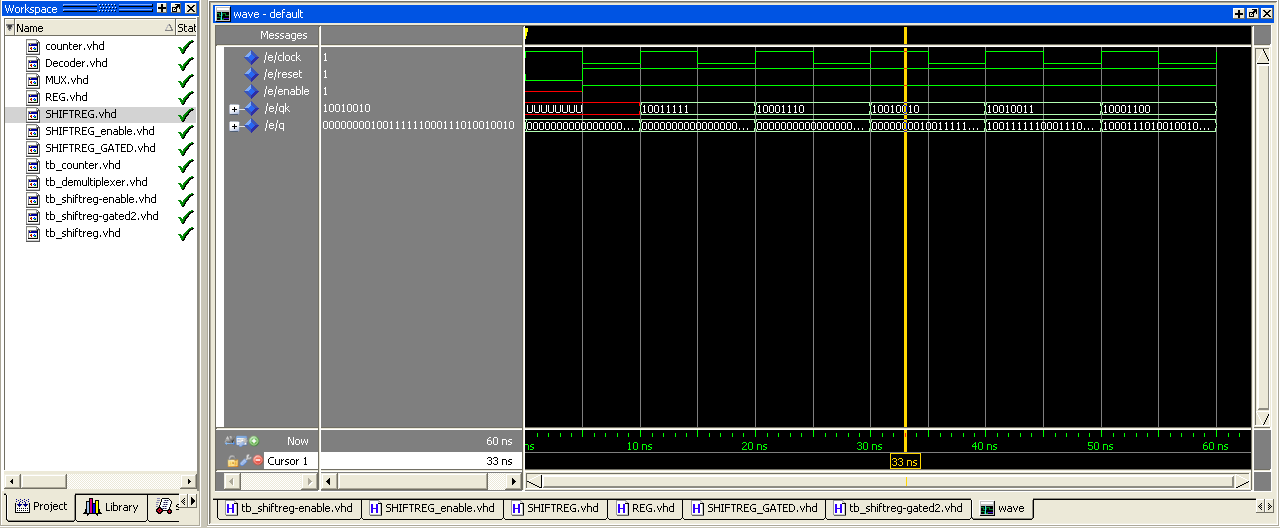
\includegraphics[length = 4in,width = 6.5in]{./images/simsr1.png}
\caption{Simulation screenshot for Design A at 33ns}
\end{figure}

\begin{figure}[htp]
\centering
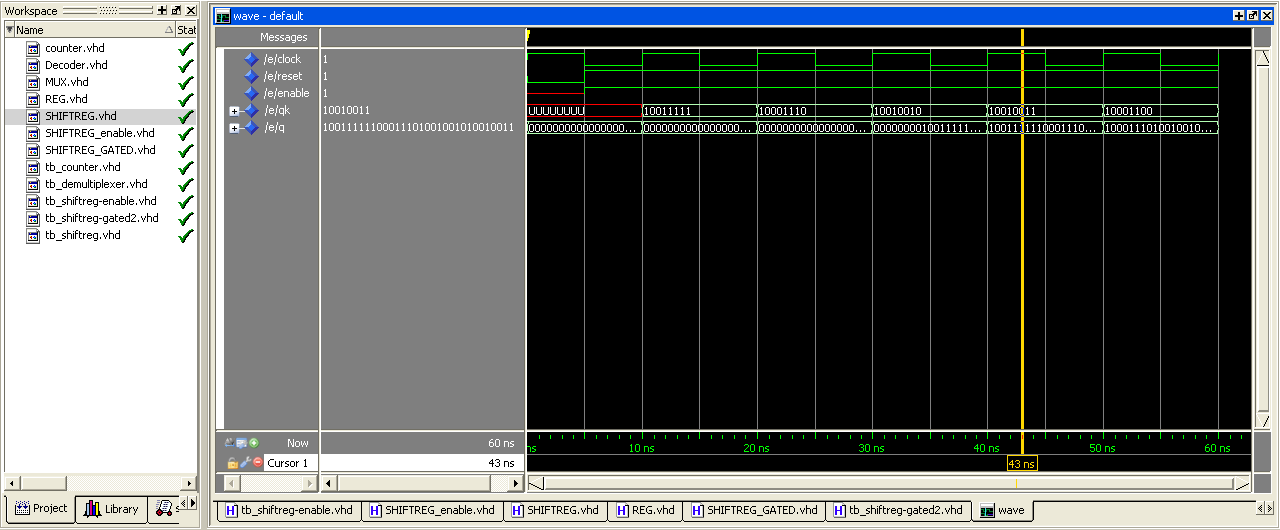
\includegraphics[length = 4in,width = 6.5in]{./images/simsr2.png}
\caption{Simulation screenshot for Design A at 43ns}
\end{figure}

\newpage
The following screenshots are from the simulation of Design B. In the first instance, at 14ns on the timeline, we have some value at Qk, but it has not been transferred in any way to the output Q. Then, at 24ns, the value of Qk in the previous clock cycle is loaded into the most significant register. Further on, at 33ns, the value of Qk in the previous clock cycle is loaded into the second most significant register. This repeats for four clock cycles, after which the most significant register is again loaded.

\begin{figure}[htp]
\centering
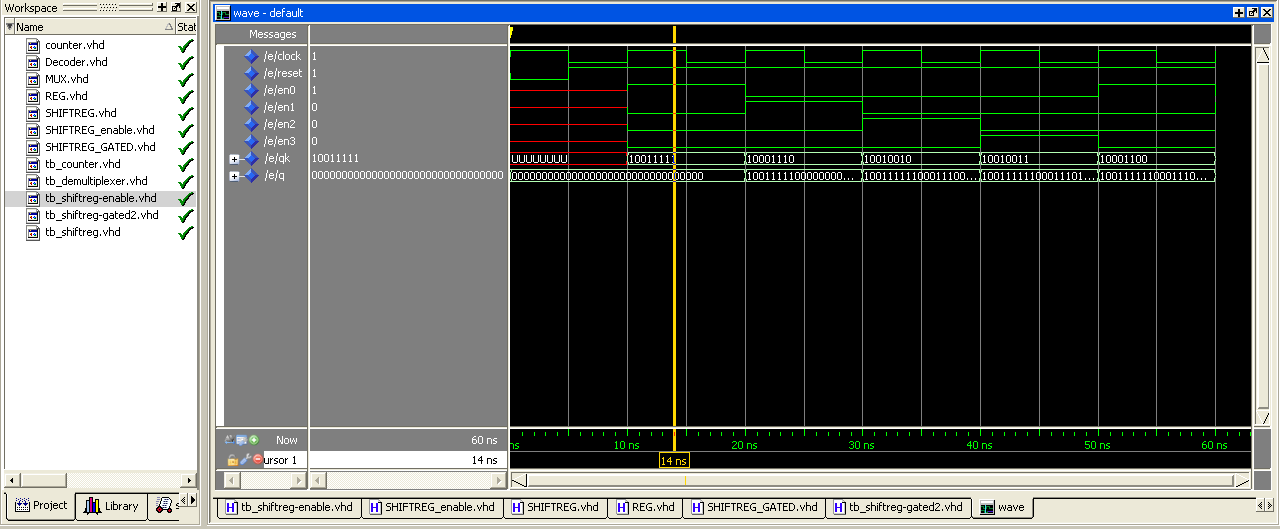
\includegraphics[length = 4in,width = 6.5in]{./images/simsre1.png}
\caption{Simulation screenshot for Design B at 14ns}
\end{figure}

\begin{figure}[htp]
\centering
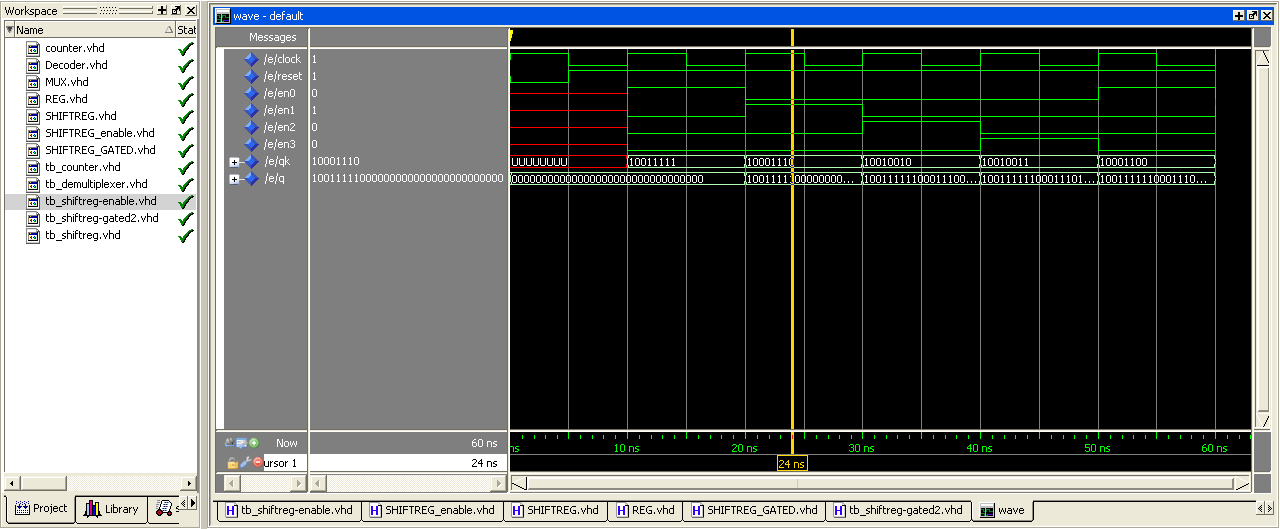
\includegraphics[length = 4in,width = 6.5in]{./images/simsre2.png}
\caption{Simulation screenshot for Design B at 24ns}
\end{figure}

\begin{figure}[htp]
\centering
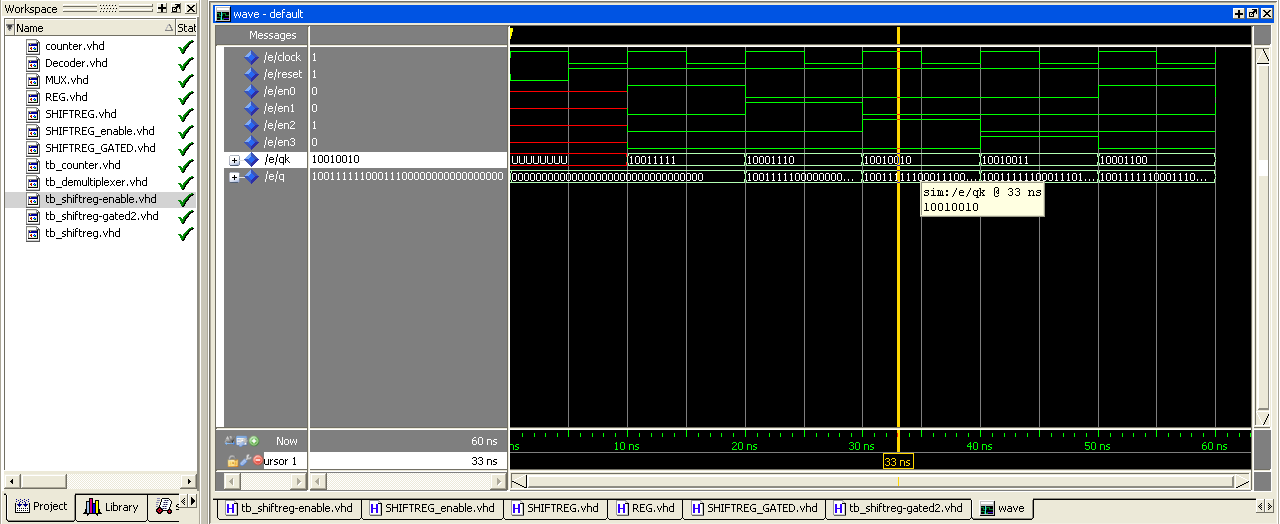
\includegraphics[length = 4in,width = 6.5in]{./images/simsre3.png}
\caption{Simulation screenshot for Design B at 33ns}
\end{figure}

\newpage
Then, for Design C, we have the following screenshots. As we can see, the values of Qk are transferred to different registers every clock cycle. This is practically the same functionality as Design B. The only difference though is that in Design C, Qk is transferred in the same clock cycle, while in Design B, it happens one clock cycle later. Ofcourse, the internal working of the two designs are completely different, which has already been discussed in section \ref{section:designs}

\begin{figure}[htp]
\centering
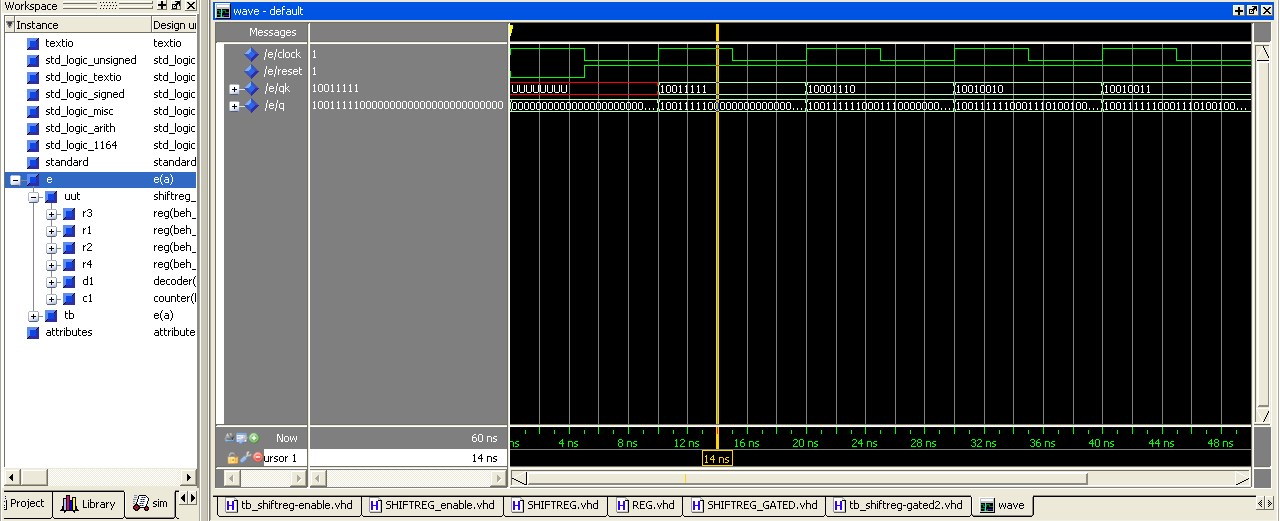
\includegraphics[length = 4in,width = 6.5in]{./images/simsrg1.png}
\caption{Simulation screenshot for Design C at 14ns}
\end{figure}

\begin{figure}[htp]
\centering
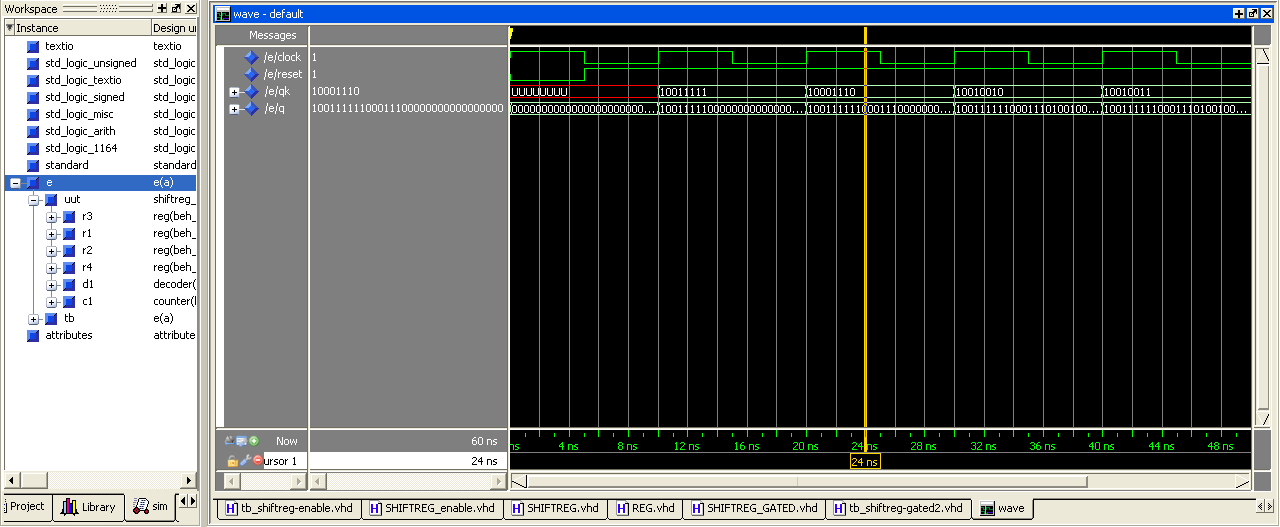
\includegraphics[length = 4in,width = 6.5in]{./images/simsrg2.png}
\caption{Simulation screenshot for Design C at 24ns}
\end{figure}

\newpage
\section{Power Reports and Discussion}
\label{section:power}

In this section we discuss the results obtained from the power-aware synthesis of the three designs. The Synopsys VSS Simulator is used to annotate the switching activity, based on a testbench for each design. This switching activity is used by Design Vision to estimate the total dynamic power consumption for the design. We have synthesized the designs for clock time periods of 2ns and 10ns and got the same results for all three designs for both clock periods. The power reports obtained from the synthesis are presented in section \ref{section:impl}. For a short recap the results can be seen in table \ref{table:power}:

%In this section we discuss the results obtained from the power-aware synthesis of the three designs. The Synopsys VSS Simulator is used to annotate the switching activity, based on a testbench for each design. This switching activity is used by Design Vision, to estimate the total dynamic power for the design. We have synthesized the designs for clock time periods of 2ns and 10ns, and have got the same results for all the three designs for the two clock periods. The power reports obtained from the synthesis are presented in section \ref{section:impl}. Though, for a short recap, the results can be seen in table \ref{table:power}:

\begin{table}[htbp]
\begin{center}
\begin{tabular}{|l|l|l|}
\hline
\textbf{}	& \textbf{Total Dynamic Power}		& \textbf{Cell Leakage Power}\\ \hline
Design A &	55.2 uW				& 773.7 nW \\ \hline
Design B &	47 uW					& 800.5 nW \\ \hline
Design C &  32.6 uW				& 835.0 nW \\ \hline
\end{tabular}
\end{center}
\caption{Overview of Results from Power Reports}
\label{table:power}
\end{table}

According to the results design A has the highest dynamic power consumption while design C has the least. We expected as much from design C, but from what we had learned on the lectures we had expected that design B would have consumed more power than design A. The static power consumption which comes from the internal leakage currents and is higher the more logic the design contains. The static power consumption is considerably lower than the dynamic power consumption in all of the designs. Because of this we will only consider the dynamic power consumption in this discussion and from now on when we use the word power we refer to the dynamic power.

In Design A the 8-bit registers change their state on each clock cycle. The input Qk is transferred from one register to the adjacent more significant register on every clock cycle until it reaches the most significant register. There it is just overwritten in the next clock cycle. Considering that only one out of four of the states of the 8-bit registers is read this kind of design is very wastful in terms of power. 75\% of the power consumed by the register state changes goes to waste. 

Design B is more efficient than Design A when it comes to the power consumed by the register state changes. Switching in Design B is controlled by the enable signals, which indicate which register should be loaded with Qk in the next clock event. If the enable signal is SET, the register is loaded with Qk, otherwise the output of the register is reloaded into the register - which consumes less power than changing the register's state. However, since the registers still consume power on each clock cycle and since the multiplexors and the logic generating their enabling signals add to the overall power consumption Design B should be less efficient than Design A when it comes to the overall power consumption. This is backed up by the lecture notes: The ratio of power dissipated in Design A to that in Design B is 1:1.19, which indicates that Design B should consume more power. We believe that the reason why our results differed from this is that the logic that generated the enabling signals was within the testbench instead of our shiftregister and thus its power dissipation fell outside of the power analysis.

Lets consider Design C now. It is quite clear that this design is most efficient from the three. This design is based on clock-gating, which means that the original clock signal is not sent directly to the registers, but sent only when the register should be loaded with a new value. So, if there is a clock signal, the register funtions normally, and power is dissipated both internally and for charging/discharging the load (if the output changes). But 75\% of the time the clock would be cut off completely, thus saving at least the internal power dissipation due to clock cycles. In Design B, even if the enable for a register was RESET, which meant that the register output would not change, there was still internal power dissipation in the cell. This is avoided in Design C since the registers do not get clock signals except when they are supposed to change their state.

We see that the attempt to reduce power disspation has been successful, without affecting the functionality of the circuit. With the reduction in power consumption comes costs in form of extra area and delay. The extra logic in designs B and C use up more area. Some delay is also added to the critical path. It should also be noted, that in Design C the rising clock edges given to the 8-bit registers come bit later than the rising edge of the actual clock signal. This means that the clock period must not be shorter than the delay or the circuit will not work properly.

%It is quite clear from the results that Design A consumes the most power (dynamic), while Design C is the most efficient, among the three designs. Though, this was expected at the beginning of the exercise. The static power, which comes from the internal leakage currents, is considerably low as compared to the dynamic power, in all the designs. So, we would not consider it in our analysis. Also, we would mean dynamic power when writing power, from now on.

%In Design A, there is a transition at the output of each of the four registers, in every clock cycle. The input Qk is transferred from one register to the adjacent more significant register, every clock cycle, until it reaches the most significant register where it is just overwritten in the next clock cycle. This is the reason why the design is much consuming in terms of power: in every clock cycle, there is a switching activity in all the output bits of the four registers. Since switching accounts for a lot of power, for the entire time line of the simulation, we have high levels of power consumption. 

%Design B is efficient than Design A. Switching in Design B is controlled by the enable signals, which indicate which register should be loaded with Qk in the next clock event. If the enable signal is SET, the register is loaded with Qk, otherwise, the output of the register remains the same. Rather, the previous value is reloaded into the register - which does have some power cost. What makes this design efficient than Design A is the reduction in the switching activity since the output of the register changes only when the enable signal is SET.

%An overhead in this design, though, is the logic for the enable signals. It is interesting to note here that we have not implemented the logic for the enable signals as a separate combinational block. The enable signals are governed from the test bench, which was provided for the exercise. Thus there is no measure of the power dissipation in the enable block, which we think would be considerable. Also, from the lecture notes, we see that the ratio of power dissipated in Design A to that in Design B is 1:1.19, which indicates that Design B should consume more power. We believe this discripancy is because the analysis does not containt the power dissipation in the logic for the enable signals.

%Lets consider Design C now. It is quite clear that this design is most efficient when compared with both Design A and Design B. This design is based on clock-gating, which means that the original clock signal is not sent directly to the registers, but sent only when the register should be loaded with a new value. So, if there is a clock signal, the register would function normally, and power is dissipated both internally and for charging/discharging the load (if the output changes). But for other cases, the clock would be cut off completely, thus saving atleast the internal power dissipation due to clock cycles. In Design B, even if the enable for a register was RESET, which meant that the register output would not change, still, since there was a clock cycle there was some power dissipated internally in the cell. This is avoided heavily in Design C.

%We see that the attempt to reduce power disspation has been successful, without affecting the functionality of the circuit. Though, with the reduction in power, there are added overheads, which cost us in area and timing. With extra logic in Design B and Design C, we need more area to accomodate the logic. And also, there is a little delay added to the critical path.



%%%% Below is the original commented out text %%%%%%%

%The results differ slightly from what we expected on the register which was implemented with multiplexers and enable signals. Otherwise the results were not surprising.

%We had expected that since the datapath was shallow, the power dissipation from the logic controlling the enabling signals and from the multiplexors would be more than the savings that are gained by eliminating unnecessary transitions in the 8-bit registers. According to these expectations the shiftregister with register enabling should have been powerhungrier than the shiftregister without register enabling. The simulation results, however, clearly show that this was not the case.

%The shiftregister with clock gating performed pretty much as we expected. We expected it to have less power dissipation than the regular shiftregister, even with the shallow datapath, since the clock control logic was simple enough not to cause more power dissipation than what is avoided by eliminating three quarters of the 8-bit register transitions.

%In our opinion the most likely reason for why the shiftregister with register enabling performed unexpectedly is the implementation of the enable signal control logic: The enable signal was controlled by logic within the test bench and was thus outside the scope of the power reports.

%Judging by the obtained results we can safely say that if low power is the number one priority (after timing of course, we want our circuit to work) then clock gating is a better method than register enabling, as clock gating gave good results even with a shallow data path. With a deeper datapath the register enabling should become a feasible option and the deeper the datapath the smaller the differences between the two techniques (powerwise) should become. Register enabling will of course demand more area than clock gating since it requires multiplexors as well as the control logic, but on higher clock frequencies clock gating can cause problems with timing because of added delay. Thus it can be said that both techniques have their uses.




\newpage
\section{Implementation and Power Reports}
\label{section:impl}

\lstinputlisting[frame=trbl, caption={SHIFTREG.vhd}]{../code/SHIFTREG.vhd}
\newpage
\lstinputlisting[frame=trbl,caption={SHIFTREG\_ENABLE.vhd}]{../code/SHIFTREG_ENABLE.vhd}
\newpage
\lstinputlisting[frame=trbl,caption={SHIFTREG\_GATED.vhd}]{../code/SHIFTREG_GATED.vhd}
\newpage
\lstinputlisting[frame=trbl,caption={REG.vhd}]{../code/REG.vhd}
\lstinputlisting[frame=trbl,caption={MUX.vhd}]{../code/MUX.vhd}
\newpage
\lstinputlisting[frame=trbl,caption={COUNTER.vhd}]{../code/counter.vhd}
\lstinputlisting[frame=trbl,caption={DECODER.vhd}]{../code/DECODER.vhd}
\newpage
\lstinputlisting[frame=trbl, caption={Power Report Design A}]{../code/power_report1.txt}
\newpage
\lstinputlisting[frame=trbl, caption={Power Report Design B}]{../code/power_report2.txt}
\newpage
\lstinputlisting[frame=trbl, , caption={Power Report Design C}]{../code/power_report3.txt}
\end{document}